\chapter{Evaluation}
\label{chap_eval}

In chapter X, Anatomy of bla bla, I concluded that the process of story­centric brainstorming and collaboration works towards the goals mentioned in the introduction section. Nonprofits have had valuable insights by working with makers, they have learned about their unique skillsets and collaborated towards solutions. Makers, in turn, practiced their skillsets and gained confidence in their abilities.

In this chapter, I focus on evaluating the move from ``real life'' collaborations to online collaborations using the newly built T  his is How platform. I start by evaluating the video medium itself and then examine the platform itself by means of comparison to the test cases presented in Chapter 3.

Video ­ Sanity Check

Before building  This is How, as a preliminary study, I tested the effectiveness of video as a medium with a group of makers. I produced several short videos telling the story of the nonprofit Cradles to Crayons, mentioned in chapter 3. This story was comprised of a two minute overview video describing the nonprofit and three short videos describing specific challenges. A static website was built, containing these videos. The webpage, along with the videos were shown to a group of makers in the South End Technology Center (SETC) in Boston.

% Figure of web page

The SETC is a makerspace, a part of the global fablab /cite{fablab} network of maker­spaces. SETC is unique in that it is operated by high school students. The students take part in a program called ``Learn to Teach, Teach to Learn'' in which they both learn fabrication skills and pass them on to the community and other students throughout the year. During the summer, the students work on projects that utilize the different skills they've learned.

I joined one of the weekly classes these students attended and presented the Cradles to Crayons story through the webpage mentioned above. The main video was shown, along with one of the challenges video. I myself did not add any information beyond the videos shown. I then opened a discussion by asking the students what they learned about the nonprofit and how they could utilize their skills to help it. Although some of the students already knew about the nonprofit, they were still surprised to learn about the complexities of running its operations. They then expressed interest in working on projects that might help in dealing with the challenges faced by the nonprofit. These project proposals beared a surprising resemblance to the ones proposed by other makers in the onsite visit described in Chapter 3.

   \begin{figure}[thpb]
      \centering
      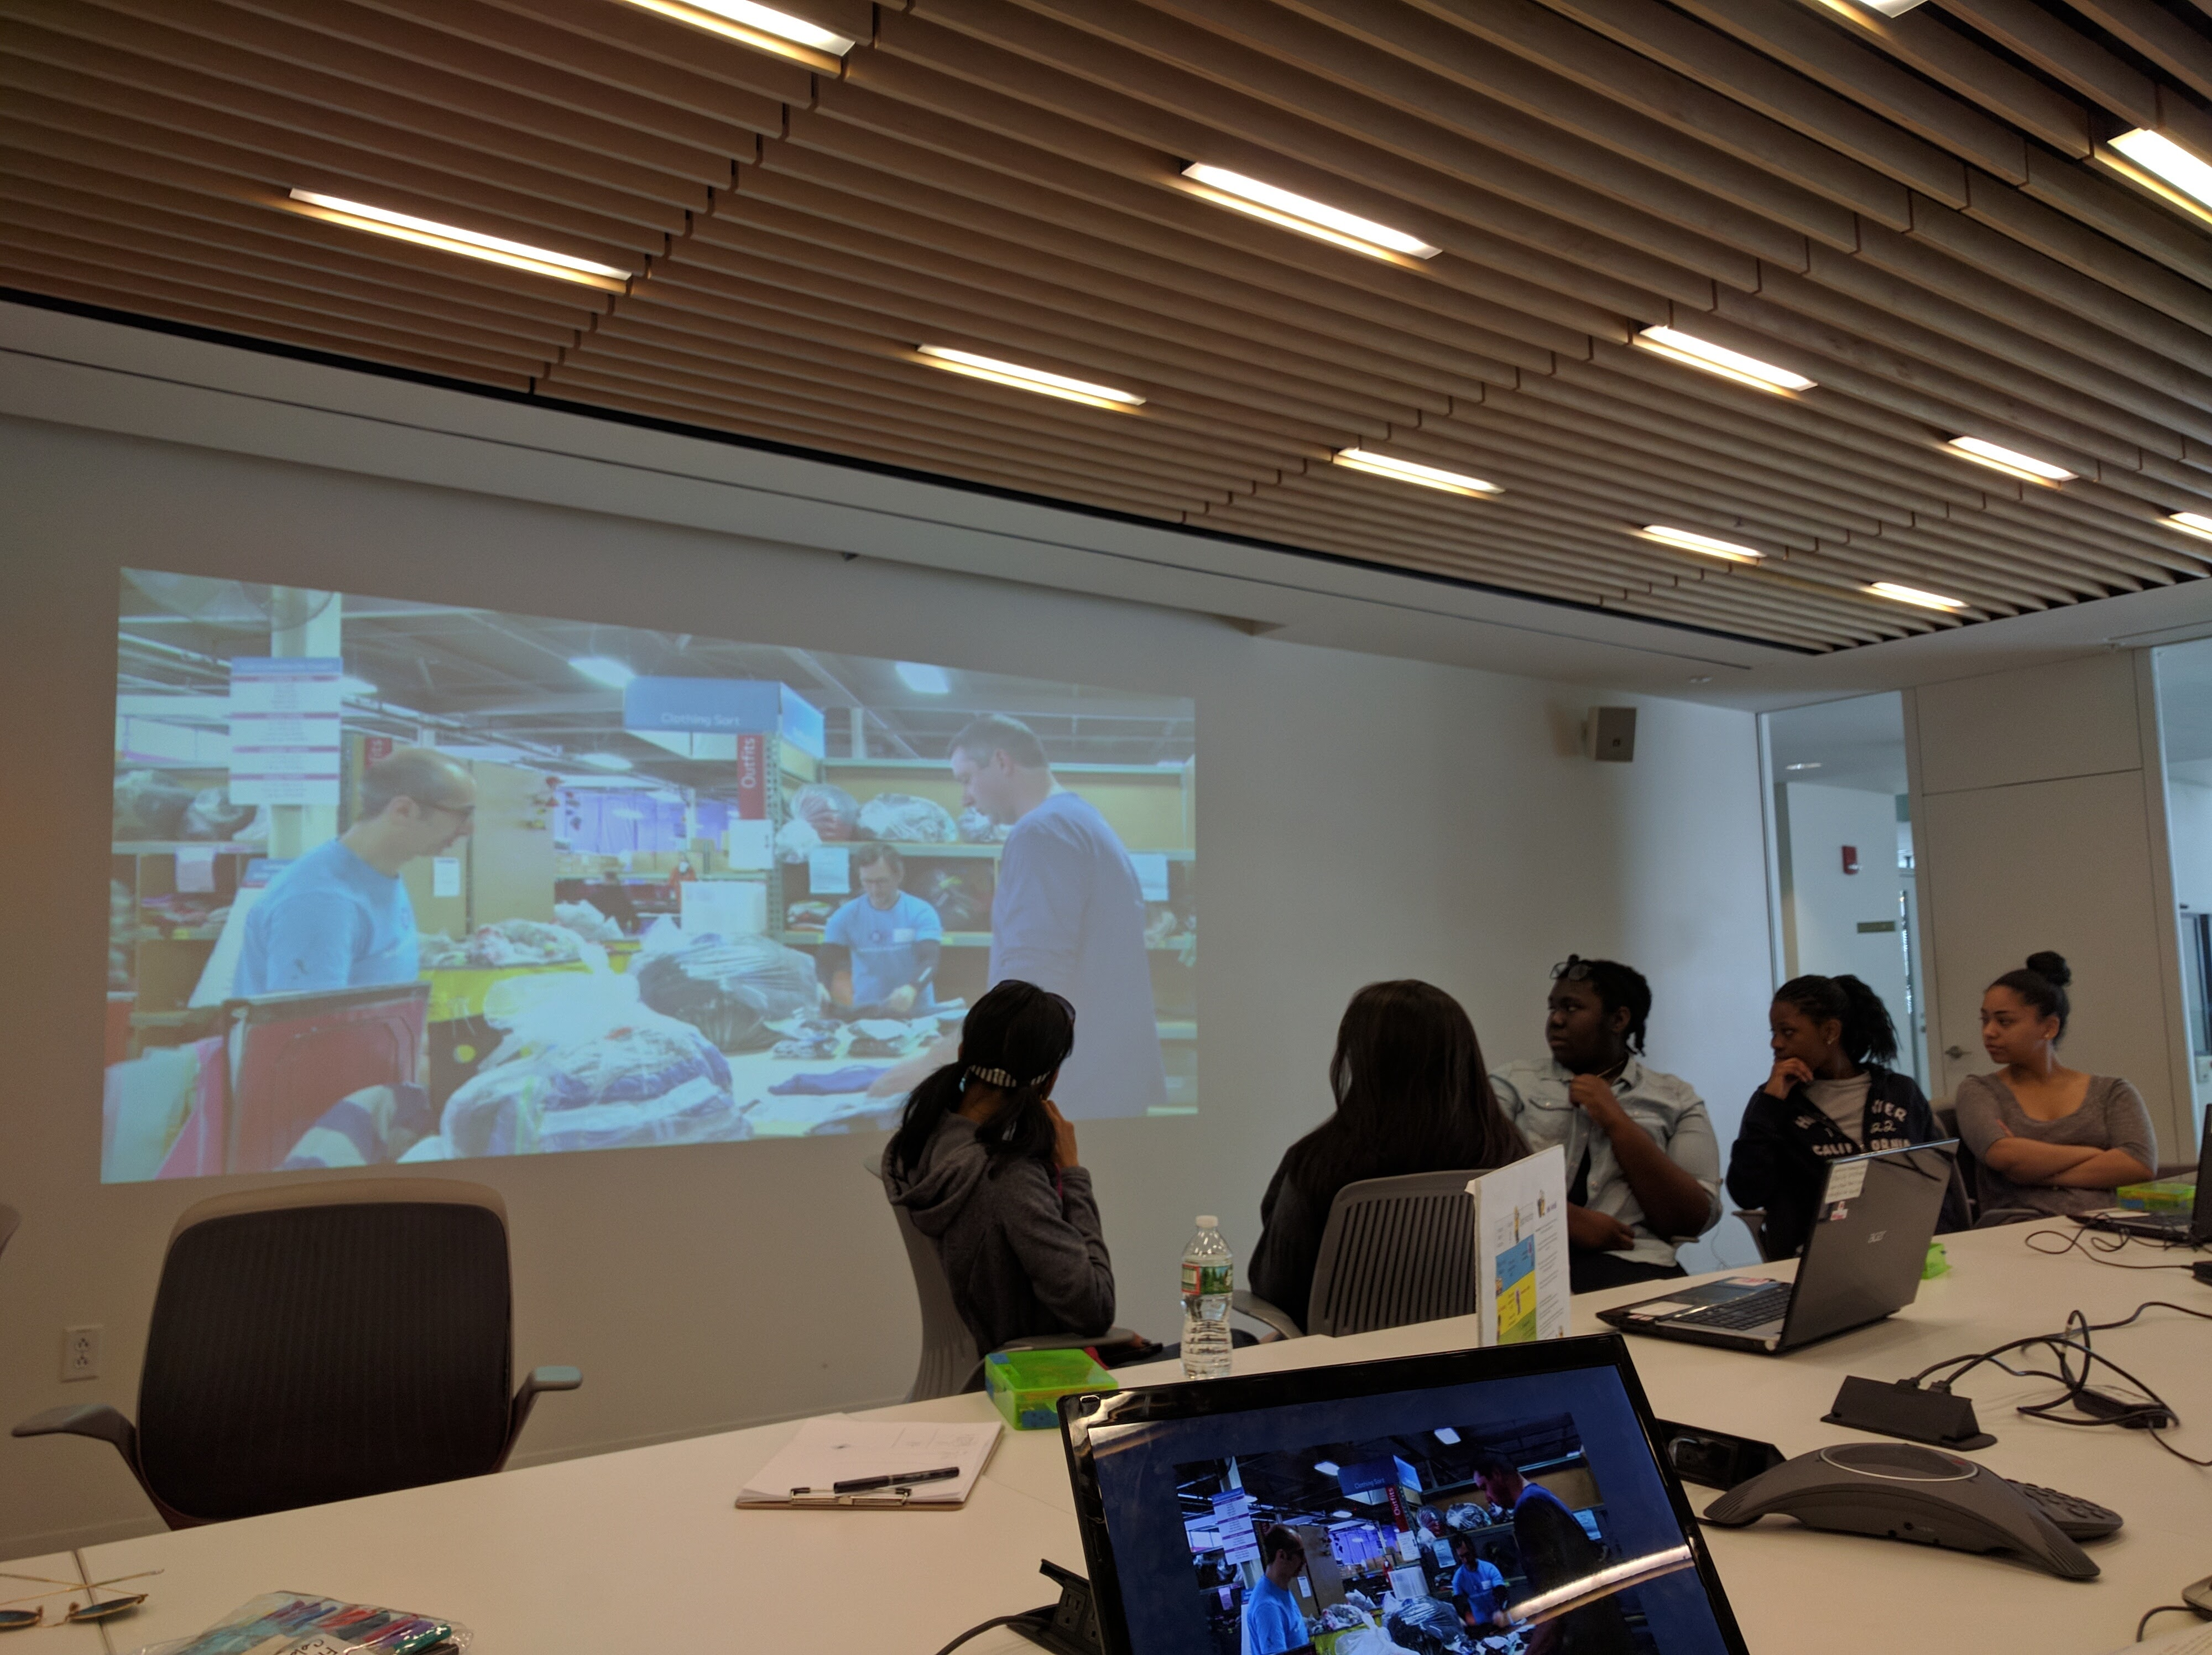
\includegraphics[width=4in]{figures/learn2teach.jpg}
      \caption{Presenting the Cradles to Crayoto story at a \textit{Learn to Teach, Teach to Learn} session}
      \label{fig_setc}
   \end{figure}

Later that day, Susan Klimczak, who runs the program, sent me an email regarding the visit which included the following:

\begin{quotation}

``When we did feedback, 5 of the youth talked about how meaningful it was to have you come in \& do the cradles to crayons! They said that it would be very valuable to have you come in regularly to present real community issues that need to be solved.''

\end{quotation}

Even without the components of interactivity and collaboration towards a solution, it was clear that the video achieved two important goals. First, it managed to raise awareness for the nonprofit, and second, it empowered the makers by providing a real world example of the value of their skills.
User Studies ­ This is How

I've conducted structured interviews (Appendix) with all three nonprofits mentioned in Chapter 3 as well as three makers who participated in some sort of collaboration with them. These nonprofits vary in scale and in type of operation.

\section{User Experience Evaluation}

The user experience evaluation centered around a demonstration given by my self. The demonstration started from the main story page, including commenting and idea pads, and then moved on to browsing and story creation. 


Per step, the interviewee was requested to rank the ease of use, according to their personal experience. They were also given an option to elaborate. I present a summary of each of the steps.

\subsection{Video}

\subsection{Story Comments System}

The subjects were shown an existing video story with comments, and comment replies, both in the form of text and video.

There was a unanimous agreement between subjects that once an existing comment in the video appears, the timeline-based discussion is self explanatory. Some of the interviewees stated that clicking on a comment to open the reply-to-comment system is not intuitive, However, once having seen it, the options to reply by text or video are self explanatory and valuable.

Makers and nonprofits alike have stated that this step seems to be true to the purpose of interactive exploration, as experienced in their collaborations. Some subjects thought the asyncronous nature of the online discussion has more potential than real life interactions because it gives the parties a chance to think about their replies. Others stated the opposite, that the asyncronous nature removes a sense of urgency which exists in real-life discussion and drives it. 

\subsection{Story Creation}

This step focused on the nonprofits, being the story creators, which all stated that the form and mechanics of uploading a file were straightforward and self explanatory, including the usage of tags as keywords. 

This step also served as a trigger for discussion regarding the feasibility of producing a compelling video story. The two smaller nonprofits stated that they believe it's within their reach to produce such a video while C2C, the largest and most established one, raised a concern regarding video quality. All media released to the public domain by them must be vetted to comply with the organization's public relation's team which has high standards.   

\subsection{Idea Pad}

The subjects were shown an Idea Pad with existing ideas regarding the same story as the previous section. Some of these ideas have already been collaborated on and discussed on by various users.

All the nonprofits stated that it is hard to evaluate without real usage although it seems to be straightforward and fits the process of brainstorming. C2C, the larger nonprofit and also the most aware of public relations, was worried that non-makers who visit the page, will not understand the goal of the idea pad.   

Two of the makers appreciated the lack of structure in the pad as a tool for free form brainstorming while the third was worried of the exact opposite, that the lack of structure does not accommodate the relationships between ideas.

\subsection{Browsing}

The subjects were shown the main page along with the option to filter by tags.

Nonprofits were neutral in their response while makers expressed a concern about scalability, how the page well look like with many stories, including the lack of a free form search option.

\subsection{Overall User Experience}

Makers and nonprofits alike have stated that in general the user interface provides a concise and self explanatory experience. The novel components, including the commenting system and the idea pad, become clear once they saw them populated with data.     


\section{"This is How" as a platform}
Subjects were asked whether they believe 